\documentclass[11pt,a4paper]{article}
\usepackage[utf8]{inputenc}
\usepackage[T1]{fontenc}
\usepackage[norsk]{babel}
\usepackage{tgtermes}
\usepackage{tgheros}
\renewcommand{\ttdefault}{txtt}
\usepackage{amsmath,amssymb}
\usepackage[a4paper,left=2.45cm,right=2.6cm,top=2.3cm,bottom=2.2cm,headsep=0.9cm]{geometry}
\usepackage{fancyhdr}
\usepackage{lastpage}
\usepackage{xcolor}
\usepackage{tikz}
\usepackage{pgfplots}
\pgfplotsset{compat=1.18}
\usepackage{booktabs}
\usepackage{array}
\usepackage{enumitem}
\usepackage{listings}
\usepackage{needspace}
\usepackage{multirow}
\usetikzlibrary{positioning,arrows.meta,calc}
\definecolor{insgrey}{gray}{0.42}
\definecolor{radiogrey}{gray}{0.70}
\setlength{\parindent}{0pt}
\setlength{\parskip}{0.45em}
\setlist[itemize]{itemsep=0pt,topsep=2pt,label=\textbullet,font=\sffamily}
\lstset{basicstyle=\ttfamily\small,columns=fullflexible,keepspaces=true,
  showstringspaces=false,upquote=true,aboveskip=0.6em,belowskip=0.6em,
  literate={æ}{{\ae}}1 {ø}{{\o}}1 {å}{{\aa}}1 {Æ}{{\AE}}1 {Ø}{{\O}}1 {Å}{{\AA}}1}
\pagestyle{fancy}
\fancyhf{}
\renewcommand{\headrulewidth}{0pt}
\fancyhead[R]{\fontsize{7.5}{9}\selectfont\sffamily\color{insgrey}TDT4172 - Introduksjon til maskinlæring - Øvingssett 5}
\fancyfoot[R]{\fontsize{7}{9}\selectfont\sffamily\color{insgrey}\thepage/\pageref{LastPage}}
\newcommand{\delstart}[1]{\clearpage
  \noindent\hspace*{-1.55em}\makebox[1.55em][l]{\sffamily\bfseries\fontsize{12}{14}\selectfont\raisebox{0.35em}{#1}}%
  {\sffamily\bfseries\fontsize{18}{22}\selectfont Part #1}\par\vspace{1.0em}}
\newcommand{\sporsmal}[1]{\par\Needspace{9\baselineskip}\vspace{1.9em}%
  \noindent{\bfseries Spørsmål #1}\par\vspace{-0.45em}%
  \noindent{\bfseries -{}-{}-{}-{}-{}-{}-{}-{}-{}-{}-{}-{}-{}-{}-{}-{}-}\par\vspace{-0.15em}}
\newcommand{\velg}[1]{\par\Needspace{6\baselineskip}\noindent{\bfseries #1}\par\vspace{0.3em}}
\newcommand{\radio}[1]{\tikz[baseline=-0.62ex]{\draw[radiogrey,line width=0.45pt,fill=gray!5] (0,0) circle (0.56em);
  \node[inner sep=0pt,font=\sffamily\fontsize{5.5}{6}\selectfont,text=insgrey] at (0,0) {#1};}}
\newenvironment{alternativer}{\begin{list}{}{\setlength{\leftmargin}{2.35em}\setlength{\labelwidth}{1.4em}%
  \setlength{\labelsep}{0.6em}\setlength{\itemsep}{0.85em}\setlength{\topsep}{0.45em}\setlength{\parsep}{0pt}}%
  \sffamily\fontsize{10}{12.6}\selectfont}{\end{list}}
\newcommand{\alt}[2]{\item[\radio{#1}]#2}
\newcommand{\makspoeng}{\par\vspace{2.2em}\hfill{\sffamily\fontsize{8.5}{10}\selectfont Maks poeng: 10}\hspace*{0.5em}\par}
\begin{document}

\noindent\hspace*{-1.55em}\makebox[1.55em][l]{\raisebox{0.3em}{\sffamily\bfseries\fontsize{11}{12}\selectfont i}}%
{\sffamily\bfseries\fontsize{18}{22}\selectfont Frontpage}\par\vspace{1.1em}

{\bfseries Eksamensoppgave i TDT4172 - Introduksjon til maskinlæring}\\
{\bfseries Øvingssett:} 5 av 10 (uoffisielt øvingssett)\\
{\bfseries Tid:} 4 timer

\vspace{0.6em}
{\bfseries Faglig kontakt:} --- (øvingssett, ikke en offisiell eksamen)\\
{\bfseries Møter i eksamenslokalet:} Nei

\vspace{0.6em}
{\bfseries Hjelpemiddelkode/Tillatte hjelpemidler:} D / Ingen trykte eller håndskrevne hjelpemidler tillatt.
Bestemt, enkel kalkulator tillatt.

\vspace{0.6em}
{\bfseries\underline{ANNEN INFORMASJON:}}

\vspace{0.4em}
{\bfseries Les oppgavene nøye og gjør dine egne antagelser.} Presiser i besvarelsen hvilke forutsetninger du
har lagt til grunn i tolkning/avgrensing av oppgaven.

Dette øvingssettet er laget for egentrening, med samme format og vanskelighetsgrad som de
siste ordinære eksamenene i emnet. Løsningsforslaget står på siste side.

\vspace{1.6em}
{\bfseries\underline{FAGSPESIFIKK INFORMASJON}}

\vspace{0.4em}
{\bfseries Ingen papirhåndtegninger:}\\
Denne eksamenen tillater ikke bruk av håndtegninger.

\vspace{1.4em}
{\bfseries Vekting av oppgavene}:\\
Denne eksamenen inneholder flervalgsoppgaver organisert i ti grupper på fire spørsmål hver. Hver
gruppe vurderes separat etter følgende regler:

\vspace{0.6em}
For hver av de fire spørsmålene i gruppen får du følgende poeng
\begin{itemize}[leftmargin=2.2em,label=\textperiodcentered,itemsep=0pt]
\item {\bfseries Riktig svar:} +2,5 poeng
\item {\bfseries Feil svar (et alternativ er valgt, men ikke korrekt):} $-$0,83 poeng
\item {\bfseries Ikke besvart:} 0 poeng
\end{itemize}
{\bfseries Merk} at dersom du først har valgt et svaralternativ, kan du {\bfseries ikke velge det bort} igjen. Da må du
svare på det spørsmålet. Med andre ord mister du muligheten til å la et spørsmål stå blankt så fort
du har trykket på et alternativ.

\vspace{0.6em}
Poengsummen for hver gruppe er {\bfseries summen} av poengene for de fire enkeltspørsmålene.\\
For {\bfseries alle spørsmålene} gjelder en {\bfseries null-grense}: dersom summen for denne gruppen blir negativ,
settes verdien til {\bfseries 0}. Den totale poengsummen på eksamen er summen av poengene fra alle
gruppene.

\delstart{1}
\sporsmal{1}
Du trener en \textbf{logistisk regresjonsmodell} med binary cross-entropy loss og gradient descent.
Du kjører treningen to ganger på nøyaktig samme treningsdata, men med ulike tilfeldige startverdier
for $\mathbf{w}$ og $b$. Læringsraten er liten nok til at begge kjøringene konvergerer.

Hva kan du forvente om de to kjøringene?
\velg{Velg ett alternativ:}
\begin{alternativer}
\alt{A}{De ender typisk i ulike lokale minima, så man bør beholde kjøringen med lavest valideringstap}
\alt{B}{De ender på ulike tapsverdier, fordi sigmoid er ikke-lineær og gir tapsflaten flere daler}
\alt{C}{De ender på samme tapsverdi bare hvis featurene er standardisert, ellers havner de i ulike minima}
\alt{D}{Begge når samme minimale tap, siden tapsfunksjonen er konveks og alle minima er globale}
\end{alternativer}
\sporsmal{2}
En logistisk regresjonsmodell for Titanic-dataene er trent til konvergens med \emph{Survived} som target
($y = 1$ betyr overlevde) og har fått parametrene $\mathbf{w}$ og $b$. En kollega trener den samme modellen på
de samme dataene, men koder target omvendt, slik at $y = 1$ betyr omkom. Tapsfunksjonen er konveks.

Hvilke parametre får kollegaens modell?
\velg{Velg ett alternativ:}
\begin{alternativer}
\alt{A}{$(\mathbf{w},\,b)$, siden kodingen av target bare påvirker tolkningen av $\hat y$}
\alt{B}{$(-\mathbf{w},\,-b)$, slik at den nye $\hat y$ blir $1 - \hat y$ for hvert punkt}
\alt{C}{$(-\mathbf{w},\,b)$, siden bare retningen på vektene snur når klassene bytter navn}
\alt{D}{$(\mathbf{w},\,-b)$, siden bare skjæringspunktet flyttes når klassene bytter navn}
\end{alternativer}
\sporsmal{3}
Du trener logistisk regresjon med gradient descent på to uskalerte features: \emph{Inntekt} (typisk
300\,000--900\,000 kr) og \emph{Alder} (20--70 år). Gradienten er $\partial L/\partial w_j = (\hat y - y)\,x_j$.
Med læringsrate $\eta = 0.01$ eksploderer tapet etter få steg, og med $\eta = 10^{-7}$ flytter vekten for
\emph{Alder} seg nesten ikke, selv etter mange epoker.

Hva er den beste forklaringen og løsningen?
\velg{Velg ett alternativ:}
\begin{alternativer}
\alt{A}{Sigmoid mettes for store input slik at gradienten forsvinner; bytt til MSE som tapsfunksjon, siden den ikke bruker sigmoid}
\alt{B}{Tapsfunksjonen blir ikke-konveks når featurene har ulik skala; prøv flere startverdier og behold kjøringen med lavest tap}
\alt{C}{Læringsraten må bare finjusteres; en verdi mellom $10^{-7}$ og $0.01$ vil gi rask konvergens for begge vektene}
\alt{D}{Gradienten for $w_{\text{Inntekt}}$ er langt større enn for $w_{\text{Alder}}$; standardiser featurene så én læringsrate passer for begge}
\end{alternativer}
\sporsmal{4}
Et datasett har disse features (target er \emph{Konvertert} og regnes ikke med):
\begin{itemize}
\item \emph{Region}: kategorisk med 5 mulige verdier
\item \emph{Abonnement}: kategorisk med verdiene \{basis, standard, premium\}
\item \emph{Daglig\_bruk}: kontinuerlig
\item \emph{Betalende}: binær \{ja, nei\}
\end{itemize}
Du one-hot-enkoder \emph{Region} og \emph{Abonnement} med én kolonne per kategori, gjør
\emph{Betalende} om til 0/1 med en LabelEncoder, og beholder \emph{Daglig\_bruk} som den er.

Hvor mange input-features får modellen?
\velg{Velg ett alternativ:}
\begin{alternativer}
\alt{A}{$8$}
\alt{B}{$10$}
\alt{C}{$6$}
\alt{D}{$4$}
\end{alternativer}
\makspoeng

\delstart{2}
\sporsmal{1}
Fire klassifiseringsmodeller er evaluert på samme valideringssett:
\begin{center}
\begin{tabular}{lcc}
\toprule
Modell & Precision & Recall \\
\midrule
M1 & 0.95 & 0.50 \\
M2 & 0.58 & 0.84 \\
M3 & 0.66 & 0.66 \\
M4 & 0.45 & 0.99 \\
\bottomrule
\end{tabular}
\end{center}
F1-score er definert som $F_1 = \dfrac{2\cdot\text{Precision}\cdot\text{Recall}}{\text{Precision}+\text{Recall}}$.

Hvilken modell har høyest \textbf{F1-score}?
\velg{Velg ett alternativ:}
\begin{alternativer}
\alt{A}{M4}
\alt{B}{M3}
\alt{C}{M2}
\alt{D}{M1}
\end{alternativer}
\sporsmal{2}
Et datasett med 12\,000 korttransaksjoner inneholder 2.5\,\% svindel. Du splitter først datasettet
\textbf{stratifisert} i 80\,\% trening og 20\,\% test. Deretter gjør du \textbf{random undersampling}
av treningsdataene slik at de to klassene blir like store.

Hvor mange datapunkter består det balanserte treningssettet av?
\velg{Velg ett alternativ:}
\begin{alternativer}
\alt{A}{$480$}
\alt{B}{$600$}
\alt{C}{$9600$}
\alt{D}{$18720$}
\end{alternativer}
\sporsmal{3}
Figuren viser ROC-kurvene til to modeller A og B på samme testsett. AUC er 0.83 for A og 0.80 for B.
\begin{center}
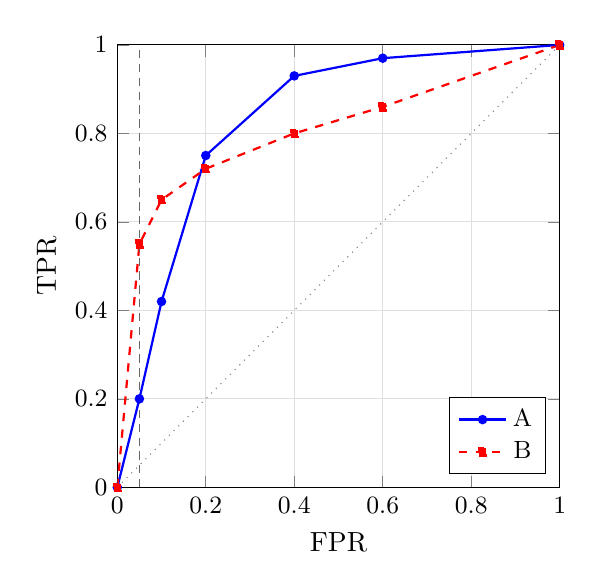
\begin{tikzpicture}
\begin{axis}[width=7.2cm,height=7.2cm,xmin=0,xmax=1,ymin=0,ymax=1,
  xlabel={FPR},ylabel={TPR},grid=major,grid style={gray!25},
  legend pos=south east,legend style={font=\small},tick label style={font=\small}]
\addplot[thick,blue,mark=*,mark size=1.3pt] coordinates {(0,0) (0.05,0.20) (0.1,0.42) (0.2,0.75) (0.4,0.93) (0.6,0.97) (1,1)};
\addlegendentry{A}
\addplot[thick,red,dashed,mark=square*,mark size=1.3pt] coordinates {(0,0) (0.05,0.55) (0.1,0.65) (0.2,0.72) (0.4,0.80) (0.6,0.86) (1,1)};
\addlegendentry{B}
\addplot[gray,dotted] coordinates {(0,0) (1,1)};
\draw[black!60,densely dashed] (axis cs:0.05,0) -- (axis cs:0.05,1);
\end{axis}
\end{tikzpicture}
\end{center}
Modellen skal brukes i et system der andelen falske alarmer blant de negative ikke kan overstige
5\,\%, altså FPR $\le 0.05$ (markert med vertikal strek).

Hvilket utsagn er riktig?
\velg{Velg ett alternativ:}
\begin{alternativer}
\alt{A}{A bør velges, siden høyest AUC gir høyest TPR ved alle FPR, også ved FPR $= 0.05$}
\alt{B}{A bør velges, siden AUC oppgir ytelsen ved den terskelen som gir FPR $= 0.05$ i drift}
\alt{C}{B bør velges, siden lavere AUC betyr færre positive prediksjoner og dermed lavere FPR}
\alt{D}{B bør velges, siden B har høyere TPR enn A ved FPR $= 0.05$, det eneste relevante driftspunktet}
\end{alternativer}
\sporsmal{4}
Svindel utgjør 1\,\% av transaksjonene. Et team oversampler svindelklassen i treningsdataene til
50/50, trener en logistisk regresjonsmodell, og bruker deretter $\hat y$ direkte som estimat på
sannsynligheten for at en ny transaksjon i drift er svindel.

Hvilket utsagn om disse estimatene er riktig?
\velg{Velg ett alternativ:}
\begin{alternativer}
\alt{A}{De blir godt kalibrerte, siden balanserte treningsdata gir de mest nøytrale sannsynlighetene}
\alt{B}{De blir typisk for høye, siden modellen er trent med en andel svindel på 50\,\% i stedet for 1\,\%}
\alt{C}{De blir typisk for lave, siden kopiene gjør at modellen overtilpasser til de få svindelpunktene}
\alt{D}{De blir uendret, siden kopiering av punkter ikke gir modellen ny informasjon om featurene}
\end{alternativer}
\makspoeng

\delstart{3}
\sporsmal{1}
En node i et beslutningstre inneholder 20 positive og 20 negative datapunkter. En kandidatsplitt gir
\begin{itemize}
\item venstre barn: 12 positive og 4 negative,
\item høyre barn: 8 positive og 16 negative.
\end{itemize}
Gini-urenheten til et datasett er $1-\sum_i p_i^2$, og urenheten etter en splitt er det vektede
gjennomsnittet over barna, vektet med andelen datapunkter i hvert barn.

Hva er Gini-urenheten etter splitten?
\velg{Velg ett alternativ:}
\begin{alternativer}
\alt{A}{$0.875$}
\alt{B}{$0.417$}
\alt{C}{$0.083$}
\alt{D}{$0.500$}
\end{alternativer}
\sporsmal{2}
To binære features $A, B \in \{0, 1\}$ bestemmer klassen slik: klassen er 1 hvis nøyaktig én av $A$ og $B$
er 1, og 0 ellers (XOR). Datasettet har 25 punkter for hver av de fire kombinasjonene av $(A, B)$.
Et beslutningstre vurderer å splitte rotnoden på $A$, med entropi $I = -\sum_i p_i\log_2 p_i$.

Hva blir informasjonsgevinsten for denne splitten, og hva betyr det?
\velg{Velg ett alternativ:}
\begin{alternativer}
\alt{A}{Gevinsten er 1, siden $A$ og $B$ til sammen bestemmer klassen fullstendig for hvert punkt}
\alt{B}{Gevinsten er 0, og en splitt på $B$ i neste nivå gir også 0, så treet kan ikke skille klassene}
\alt{C}{Gevinsten er 0, og et tre som splitter på $A$ og deretter på $B$ klassifiserer alle punktene riktig}
\alt{D}{Gevinsten er 0.5, men den stiger til 1 når $B$ brukes som splitt i neste nivå av treet}
\end{alternativer}
\sporsmal{3}
Du trener et \texttt{DecisionTreeClassifier} uten dybdebegrensning to ganger med de samme
hyperparametrene: først på alle 500 treningspunktene, og deretter etter å ha fjernet fem tilfeldige
punkter. Det første treet splitter rotnoden på \emph{Alder}, det andre på \emph{Inntekt}, og resten av
de to trærne er helt forskjellige.

Hva er den beste forklaringen?
\velg{Velg ett alternativ:}
\begin{alternativer}
\alt{A}{To kandidatsplitter var nesten like gode i rotnoden, og når valget bytter, endres alle splittene under}
\alt{B}{Dype trær har høy bias, og høy bias gjør at små endringer i dataene gir et helt annet tre}
\alt{C}{Treet starter fra tilfeldige startverdier for vektene, så to treninger gir ulike trær selv på samme data}
\alt{D}{Fjerningen endret skalaen til featurene, og splittvalget i et beslutningstre er følsomt for skalering}
\end{alternativer}
\sporsmal{4}
En sykdom forekommer hos 1\,\% av befolkningen. En test gir positivt svar hos 95\,\% av de syke, og
hos 10\,\% av de friske.

En tilfeldig valgt person tester positivt. Omtrent hvor stor er sannsynligheten for at personen er syk?
\velg{Velg ett alternativ:}
\begin{alternativer}
\alt{A}{ca. 8.8\,\%}
\alt{B}{ca. 95\,\%}
\alt{C}{ca. 90\,\%}
\alt{D}{ca. 10.9\,\%}
\end{alternativer}
\makspoeng

\delstart{4}
\sporsmal{1}
Du tilpasser polynomer av grad 2, 4, 8 og 12 (features $x, x^2, \dots, x^M$) til de \textbf{samme}
treningsdataene med gradient descent på MSE, og måler tapet på treningsdataene:
\begin{center}
\begin{tabular}{lcccc}
\toprule
Grad $M$ & 2 & 4 & 8 & 12 \\
Trenings-MSE & 9.6 & 3.2 & 2.5 & 3.0 \\
\bottomrule
\end{tabular}
\end{center}
En kollega mener at økningen fra grad 8 til grad 12 viser at modellen overtilpasser.
Hvilket utsagn er riktig?
\velg{Velg ett alternativ:}
\begin{alternativer}
\alt{A}{Økningen skyldes tilfeldig variasjon i datasplitten og ville forsvunnet med k-fold kryssvalidering}
\alt{B}{Kollegaen har rett; overtilpasning vises ved at trenings-MSE begynner å øke når graden blir for høy}
\alt{C}{Økningen er ventet, siden flere ledd gir høyere bias, og biasen dominerer feilen på treningsdataene}
\alt{D}{En modell av grad 12 rommer alle modeller av grad 8, så optimeringen har stanset før minimum er nådd}
\end{alternativer}
\sporsmal{2}
Du har 1000 datapunkter og vil sammenligne 4 ulike verdier av en hyperparameter med
\textbf{5-fold kryssvalidering}.

Hvilket utsagn er riktig?
\velg{Velg ett alternativ:}
\begin{alternativer}
\alt{A}{Totalt trenes 20 modeller, og hver av dem valideres på 800 datapunkter som ikke ble brukt i treningen}
\alt{B}{Totalt trenes 20 modeller, og hvert datapunkt brukes til validering i fire av de fem foldene}
\alt{C}{Totalt trenes 20 modeller, og hvert punkt brukes til validering nøyaktig én gang per hyperparameterverdi}
\alt{D}{Totalt trenes 5 modeller, fordi alle hyperparameterverdiene kan evalueres på samme modell i hver fold}
\end{alternativer}
\sporsmal{3}
Både \textbf{bootstrapping} og \textbf{$k$-fold kryssvalidering} lager flere delsett fra ett datasett med
$n$ punkter.

Hvilket utsagn beskriver riktig hvordan delsettene skiller seg?
\velg{Velg ett alternativ:}
\begin{alternativer}
\alt{A}{Bootstrap trekker uten tilbakelegging, så utvalgene kan overlappe, men ingen punkter gjentas i ett utvalg}
\alt{B}{Bootstrap trekker med tilbakelegging, men hvert punkt havner likevel i bare ett utvalg, som i $k$-fold}
\alt{C}{Bootstrap-utvalgene kan overlappe og inneholde duplikater, mens foldene i $k$-fold er disjunkte}
\alt{D}{Begge lager disjunkte delsett, men bootstrap bruker flere delsett enn $k$-fold og gir lavere varians}
\end{alternativer}
\sporsmal{4}
Modellen $f(x) = \beta_0 + \beta_1 x$ trenes med gradient descent på
$\text{MSE} = \frac{1}{2N}\sum_{i}\bigl(y^{(i)} - f(x^{(i)})\bigr)^2$, slik at
\[
\frac{\partial L}{\partial \beta_0} = \frac{1}{N}\sum_{i=1}^{N}\bigl(f(x^{(i)}) - y^{(i)}\bigr).
\]
Treningsdataene er
\begin{center}
\begin{tabular}{ccccc}
\toprule
$x$ & 1 & 2 & 4 & 5 \\
$y$ & 4 & 5 & 10 & 11 \\
\bottomrule
\end{tabular}
\end{center}
Anta at stigningstallet er ferdig tilpasset og holdes fast på $\beta_1 = 2$.
Hvilken verdi av $\beta_0$ gjør $\partial L/\partial\beta_0 = 0$?
\velg{Velg ett alternativ:}
\begin{alternativer}
\alt{A}{$1.50$}
\alt{B}{$4.50$}
\alt{C}{$7.50$}
\alt{D}{$6.00$}
\end{alternativer}
\makspoeng

\delstart{5}
\sporsmal{1}
Gradient boosting for regresjon brukes på tre datapunkter med targets $y = (10,\,14,\,18)$.
Startprediksjonen er gjennomsnittet, $F_0(x) = 14$ for alle punkter. I hver runde $m$ tilpasses et
nytt tre $h_m$ til pseudo-residualene $r = y - F_{m-1}(x)$, og vi antar at treet treffer dem eksakt.
Ensemblet oppdateres med læringsrate $\eta = 0.1$:
\[
F_m(x) = F_{m-1}(x) + \eta\, h_m(x).
\]

Hva er prediksjonen $F_2$ for punktet med $y = 18$ etter to runder?
\velg{Velg ett alternativ:}
\begin{alternativer}
\alt{A}{$14.76$}
\alt{B}{$18.00$}
\alt{C}{$14.80$}
\alt{D}{$13.16$}
\end{alternativer}
\sporsmal{2}
Et treningssett inneholder noen få punkter med \textbf{feilregistrert label}. Du trener AdaBoost med
trestumper, og ser at disse punktene klassifiseres feil av nesten hver ny stump, runde etter runde.

Hva skjer med disse punktene, og hva betyr det for ensemblet?
\velg{Velg ett alternativ:}
\begin{alternativer}
\alt{A}{Vektene deres blir stadig større, men det påvirker bare treningsfeilen og ikke prediksjonene på nye data}
\alt{B}{Vektene deres endres ikke, siden vektene bare justeres for punktene som den første stumpen bommet på}
\alt{C}{Vektene deres blir stadig større, så senere stumper bruker mye av kapasiteten sin på å tilpasse seg støy}
\alt{D}{Vektene deres settes til null etter noen runder, siden AdaBoost oppdager at punktene er umulige å lære}
\end{alternativer}
\sporsmal{3}
Du trener gradient boosting for regresjon med kvadratisk tap og læringsrate $\eta = 1$. Ved en feil settes
maks dybde så høyt at det første treet etter startprediksjonen tilpasser treningsdataene perfekt, slik at
trenings-MSE blir 0.

Hva skjer i de påfølgende boosting-rundene?
\velg{Velg ett alternativ:}
\begin{alternativer}
\alt{A}{Neste tre får høyere vekt på de vanskeligste punktene, slik at overtilpasningen gradvis rettes opp}
\alt{B}{Pseudo-residualene er 0, så neste tre tilpasses i stedet de opprinnelige targetene på nytt}
\alt{C}{Pseudo-residualene er 0 for alle treningspunkter, så nye trær predikerer 0 og ensemblet endres ikke}
\alt{D}{Neste tre tilpasses de største feilene på valideringsdata, slik at ensemblet gradvis generaliserer bedre}
\end{alternativer}
\sporsmal{4}
Du har et treningssett med $n = 1000$ punkter og trener et \textbf{bagging}-ensemble med 50 beslutningstrær.

Hvilken beskrivelse av treningsdataene til tre nummer 17 er riktig?
\velg{Velg ett alternativ:}
\begin{alternativer}
\alt{A}{De 1000 punktene i ny tilfeldig rekkefølge, slik at forskjellen mellom trærne skyldes rekkefølgen}
\alt{B}{1000 punkter trukket med tilbakelegging, der punktene tre 16 bommet på har høyere sannsynlighet for å bli trukket}
\alt{C}{20 punkter, slik at de 50 trærne til sammen deler treningssettet i disjunkte deler}
\alt{D}{1000 punkter trukket med tilbakelegging, så noen punkter forekommer flere ganger og andre mangler}
\end{alternativer}
\makspoeng

\delstart{6}
\sporsmal{1}
Et nevralt nettverk trenes på $N = 8000$ treningspunkter i 5 epoker.

Hvor mange parameteroppdateringer gjør henholdsvis \textbf{SGD} (ett datapunkt per oppdatering) og
\textbf{mini-batch SGD} med batch size $B = 50$ i løpet av de 5 epokene?
\velg{Velg ett alternativ:}
\begin{alternativer}
\alt{A}{SGD: $8\,000$, mini-batch: $250$}
\alt{B}{SGD: $40\,000$, mini-batch: $800$}
\alt{C}{SGD: $8\,000$, mini-batch: $800$}
\alt{D}{SGD: $40\,000$, mini-batch: $250$}
\end{alternativer}
\sporsmal{2}
Du trener et nevralt nettverk med mini-batch SGD og vurderer å endre \textbf{batch size} fra 256 til 16.

Hvilket utsagn er riktig?
\velg{Velg ett alternativ:}
\begin{alternativer}
\alt{A}{Med 16 blir gradientestimatet mer presist, fordi hvert datapunkt får større innflytelse på oppdateringen}
\alt{B}{Batch size er en modellparameter som justeres med backpropagation sammen med vektene og biasene i nettverket}
\alt{C}{Batch size påvirker hvor lang tid en epoke tar, men oppdateringene blir de samme uansett batch size}
\alt{D}{Batch size er en hyperparameter; med 16 blir gradienten mer støyete, men hver oppdatering billigere}
\end{alternativer}
\sporsmal{3}
Et nettverk har to inputs, ett skjult lag med to ReLU-noder $(h_1, h_2)$ og én sigmoid-node i output-laget, og er
trent til nesten 100\,\% accuracy på et binært problem der klassene \textbf{ikke} er lineært separerbare i
$(x_1, x_2)$. Når du plotter aktiveringene $(h_1, h_2)$ for treningspunktene, kan de to klassene skilles med en
rett linje i $(h_1, h_2)$-planet.

Hva er den beste tolkningen?
\velg{Velg ett alternativ:}
\begin{alternativer}
\alt{A}{Det skjulte laget har lært en rotasjon og skalering av input, slik PCA gjør, uten ikke-linearitet}
\alt{B}{Sigmoid i output-noden gir den ikke-lineære grensen, mens det skjulte laget bare skalerer input}
\alt{C}{Det skjulte laget har lært nye features, og output-noden er en logistisk regresjon på dem}
\alt{D}{Nettverket har trolig overtilpasset, siden lineær separerbarhet i $(h_1, h_2)$ krever at punktene er pugget}
\end{alternativer}
\sporsmal{4}
Et perceptron for tre klasser har to inputs og én output-node per klasse, alle med Heaviside-aktivering.
Vektene oppdateres med
\[
w_{i,j} \leftarrow w_{i,j} + \eta\,(y_j - \hat y_j)\,x_i ,
\]
der $w_{i,j}$ er vekten fra input $i$ til output-node $j$. For datapunktet $\mathbf{x} = (2,\,-1)$ med
target $\mathbf{y} = (0,\,0,\,1)$ gir perceptronet $\hat{\mathbf{y}} = (1,\,0,\,1)$, og $\eta = 0.5$.
Se bort fra bias.

Hvilken endring gjøres i vektene?
\velg{Velg ett alternativ:}
\begin{alternativer}
\alt{A}{Ingen vekter endres, siden node 3 er aktiv og perceptronet dermed allerede gir riktig klasse}
\alt{B}{Vektene inn til node 1 og 3 endres, med $(-1.0,\,+0.5)$ for node 1 og $(+1.0,\,-0.5)$ for node 3}
\alt{C}{Bare vektene inn til node 1 endres, med $(\Delta w_{1,1},\,\Delta w_{2,1}) = (+1.0,\,-0.5)$}
\alt{D}{Bare vektene inn til node 1 endres, med $(\Delta w_{1,1},\,\Delta w_{2,1}) = (-1.0,\,+0.5)$}
\end{alternativer}
\makspoeng

\delstart{7}
\sporsmal{1}
Figuren viser et datasett som består av to konsentriske ringer. Fargene viser resultatet av
\textbf{k-means} med $k=2$: dataene er delt i en venstre og en høyre halvdel.
\begin{center}
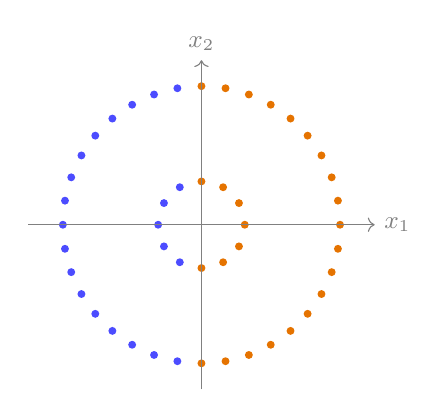
\begin{tikzpicture}[scale=0.55]
\foreach \a in {0,30,...,330} {
  \pgfmathsetmacro{\cosv}{cos(\a)}
  \ifdim \cosv pt < -0.01pt
    \fill[blue!70] ({cos(\a)},{sin(\a)}) circle (2.6pt);
  \else
    \fill[orange!90!black] ({cos(\a)},{sin(\a)}) circle (2.6pt);
  \fi
}
\foreach \a in {0,10,...,350} {
  \pgfmathsetmacro{\cosv}{cos(\a)}
  \ifdim \cosv pt < -0.01pt
    \fill[blue!70] ({3.2*cos(\a)},{3.2*sin(\a)}) circle (2.6pt);
  \else
    \fill[orange!90!black] ({3.2*cos(\a)},{3.2*sin(\a)}) circle (2.6pt);
  \fi
}
\draw[->,gray] (-4,0) -- (4,0) node[right] {\small $x_1$};
\draw[->,gray] (0,-3.8) -- (0,3.8) node[above] {\small $x_2$};
\end{tikzpicture}
\end{center}

Hvorfor finner ikke k-means de to ringene?
\velg{Velg ett alternativ:}
\begin{alternativer}
\alt{A}{Featurene er ikke skalert; etter standardisering ville avstandene trolig skilt den indre og ytre ringen}
\alt{B}{k-means tilordner punkter til nærmeste sentroide og antar dermed kompakte, omtrent sfæriske klynger}
\alt{C}{k-means krever like mange punkter i hver klynge, og den ytre ringen inneholder flere punkter enn den indre}
\alt{D}{Initialiseringen var uheldig; med k-means++ ville sentroidene havnet slik at ringene ble skilt}
\end{alternativer}
\sporsmal{2}
Du skal klynge 20 millioner GPS-posisjoner med to features og vurderer k-means og DBSCAN.
Beregningstid er det viktigste kriteriet.

Hvilket utsagn er riktig?
\velg{Velg ett alternativ:}
\begin{alternativer}
\alt{A}{DBSCAN skalerer best, fordi k-means må beregne avstanden mellom alle par av datapunkter i hver iterasjon}
\alt{B}{DBSCAN skalerer best, fordi den ikke trenger antall klynger og derfor slipper å kjøres for mange verdier av $k$}
\alt{C}{k-means skalerer best, fordi DBSCAN må kjøres på nytt for hver kombinasjon av $\varepsilon$ og \texttt{min\_samples}}
\alt{D}{k-means skalerer best, fordi DBSCAN må finne naboene til hvert punkt og dermed beregne avstander mellom svært mange par}
\end{alternativer}
\sporsmal{3}
Etter en clustering beregner du silhouette-koeffisienten $s = (b-a)/\max(a,b)$ for hvert punkt, der $a$ er
midlere avstand til de andre punktene i egen klynge og $b$ er midlere avstand til punktene i nærmeste
andre klynge. Punktet P får $s = -0.4$.

Hva forteller dette om P?
\velg{Velg ett alternativ:}
\begin{alternativer}
\alt{A}{P er trolig en outlier, siden en negativ verdi betyr at P ligger langt fra alle klyngene}
\alt{B}{P ligger på grensen mellom to klynger, siden negative verdier betyr at klyngene overlapper}
\alt{C}{P ligger i snitt nærmere den andre klyngen enn sin egen, og er trolig i feil klynge}
\alt{D}{P er rimelig godt plassert, siden bare absoluttverdien $|s| = 0.4$ har betydning}
\end{alternativer}
\sporsmal{4}
k-means med $k=2$ kjøres på seks punkter i planet:
\[
(1,1),\ (2,1),\ (1,2),\ (3,2),\ (4,3),\ (5,4).
\]
Startsentroidene er $\mathbf{c}_1 = (1,1)$ og $\mathbf{c}_2 = (5,4)$, og det brukes Euklidsk avstand.

Hva blir de nye sentroidene etter ett tilordningssteg og ett oppdateringssteg?
\velg{Velg ett alternativ:}
\begin{alternativer}
\alt{A}{$\mathbf{c}_1 = (1.75,\,1.50)$ og $\mathbf{c}_2 = (4.50,\,3.50)$}
\alt{B}{$\mathbf{c}_1 = (1.60,\,1.40)$ og $\mathbf{c}_2 = (4.67,\,3.67)$}
\alt{C}{$\mathbf{c}_1 = (1.33,\,1.33)$ og $\mathbf{c}_2 = (4.00,\,3.00)$}
\alt{D}{$\mathbf{c}_1 = (2.00,\,1.50)$ og $\mathbf{c}_2 = (4.50,\,3.50)$}
\end{alternativer}
\makspoeng

\delstart{8}
\sporsmal{1}
Du lager t-SNE-plott av samme datasett med \texttt{perplexity=3} og med \texttt{perplexity=50}.

Hvilket utsagn om \textbf{perplexity} er riktig?
\velg{Velg ett alternativ:}
\begin{alternativer}
\alt{A}{Den er antall frihetsgrader i t-fordelingen og kan tolkes som hvor tunge halene i det lavdimensjonale rommet er}
\alt{B}{Den styrer variansen til gaussen rundt hvert punkt og kan tolkes som effektivt antall naboer}
\alt{C}{Den angir antall dimensjoner i embeddingen, slik at \texttt{perplexity=3} gir en tredimensjonal embedding}
\alt{D}{Den angir antall iterasjoner med gradient descent, så høy perplexity gir en bedre konvergert embedding}
\end{alternativer}
\sporsmal{2}
t-SNE minimerer \textbf{KL-divergensen}
$D_{KL}(P\,\|\,Q) = \sum_x P(x)\log\dfrac{P(x)}{Q(x)}$ mellom naboskapsfordelingene $P$ (høydimensjonalt)
og $Q$ (lavdimensjonalt).

Hvilket utsagn om KL-divergensen er riktig?
\velg{Velg ett alternativ:}
\begin{alternativer}
\alt{A}{Den er aldri negativ, og $D_{KL}(P\|Q) = D_{KL}(Q\|P)$, slik at den er et avstandsmål som Euklidsk avstand}
\alt{B}{Den er aldri negativ og er 0 når $P = Q$, men $D_{KL}(P\|Q)$ og $D_{KL}(Q\|P)$ er generelt ulike}
\alt{C}{Den er symmetrisk i $P$ og $Q$, men kan bli negativ når $Q$ er mer konsentrert enn $P$}
\alt{D}{Den er 0 når $P$ og $Q$ har lik varians, men vokser ellers med forskjellen i varians mellom dem}
\end{alternativer}
\sporsmal{3}
Du har 20\,000 kunder med 50 features og to ønsker:
\begin{itemize}
\item[(1)] et 2D-plott der kunder med lignende profil havner tett sammen i tydelige grupper,
\item[(2)] et tall for hvor stor andel av den totale variansen som bevares i to dimensjoner.
\end{itemize}
Hvilken kombinasjon passer best?
\velg{Velg ett alternativ:}
\begin{alternativer}
\alt{A}{t-SNE for (1), siden den bevarer lokale nabolag, og PCA for (2), siden egenverdiene gir variansandelen}
\alt{B}{PCA for (1), siden den bevarer lokale nabolag, og t-SNE for (2), siden KL-divergensen gir variansandelen}
\alt{C}{t-SNE for begge, siden KL-divergensen etter treningen angir hvor stor andel av variansen som er bevart}
\alt{D}{PCA for begge, siden t-SNE også er en lineær projeksjon og derfor ikke kan vise grupper bedre enn PCA}
\end{alternativer}
\sporsmal{4}
Kovariansmatrisen til et sentrert datasett med to features er
\[
S = \begin{pmatrix} 5 & 2 \\ 2 & 2 \end{pmatrix}.
\]

Hvilken retning har første hovedkomponent (PC1), og hvor stor er variansen til dataene langs PC1?
\velg{Velg ett alternativ:}
\begin{alternativer}
\alt{A}{PC1 $\propto (1,\,-2)$, og variansen langs PC1 er $1$}
\alt{B}{PC1 $\propto (2,\,1)$, og variansen langs PC1 er $6$}
\alt{C}{PC1 $\propto (2,\,1)$, og variansen langs PC1 er $1$}
\alt{D}{PC1 $\propto (1,\,-2)$, og variansen langs PC1 er $6$}
\end{alternativer}
\makspoeng

\delstart{9}
\sporsmal{1}
I Q-læring tar agenten handlingen $A_t$ i tilstanden $S_t$, får belønningen $R_{t+1} = 1$, og
miljøet returnerer \texttt{done=True} fordi agenten har nådd målet og episoden er over.

Hvordan bør target-verdien i Q-oppdateringen for $(S_t, A_t)$ beregnes?
\velg{Velg ett alternativ:}
\begin{alternativer}
\alt{A}{Som $R_{t+1}/(1-\gamma)$, fordi agenten antas å få samme belønning i alle fremtidige steg etter målet}
\alt{B}{Som bare $R_{t+1}$, fordi en terminaltilstand ikke har fremtidig verdi og $\gamma\max_A Q(S_{t+1},A)$ settes til 0}
\alt{C}{Som $R_{t+1} + \gamma\max_A Q(S_{t+1},A)$ som vanlig, fordi Q-verdiene i terminaltilstanden læres som for andre tilstander}
\alt{D}{Som 0, fordi episoden er over og belønningen i siste steg derfor ikke kan påvirke Q-verdiene lenger}
\end{alternativer}
\sporsmal{2}
Du trener en Q-agent med epsilon decay, og $\epsilon$ når \texttt{epsilon\_min} etter omtrent 1500 episoder.
Etter 3000 episoder har agenten fortsatt nesten aldri nådd målet, og total reward per episode har ikke
økt i løpet av treningen.

Hva er det mest fornuftige neste steget?
\velg{Velg ett alternativ:}
\begin{alternativer}
\alt{A}{Endre andre deler av oppsettet, for eksempel reward eller tapsfunksjon, før du trener på nytt}
\alt{B}{Tren videre i mange flere episoder, siden Q-verdiene trenger tid etter at utforskingen er over}
\alt{C}{Sett $\epsilon = 0$ resten av treningen, slik at agenten kan utnytte det den har lært til nå}
\alt{D}{Senk $\gamma$, slik at agenten vektlegger umiddelbar reward og dermed lærer raskere}
\end{alternativer}
\sporsmal{3}
Et miljø har omtrent $10^{12}$ mulige tilstander, og agenten vil bare besøke en liten brøkdel av dem
under treningen.

Hvorfor er et DQN bedre egnet enn en Q-tabell her?
\velg{Velg ett alternativ:}
\begin{alternativer}
\alt{A}{Et nettverk generaliserer fra lignende tilstander, så det gir Q-verdier også der en tabell er tom}
\alt{B}{Et DQN lagrer Q-verdiene i en replay buffer i stedet for i en tabell, og trenger derfor mindre minne}
\alt{C}{Et DQN trenger ikke utforsking, siden nettverket predikerer Q-verdiene uten å prøve handlingene}
\alt{D}{Et DQN gir mer stabil trening enn en tabell, fordi én oppdatering justerer mange Q-verdier samtidig}
\end{alternativer}
\sporsmal{4}
En robotstøvsuger trenes med reinforcement learning. I hvert tidssteg $t$ har systemet en
tilstand $S_t$, en handling $A_t$ og en belønning $R_{t+1}$.

Hvilket utsagn beskriver rollene i \textbf{RL-loopen} riktig?
\velg{Velg ett alternativ:}
\begin{alternativer}
\alt{A}{Miljøet velger $A_t$ ut fra $S_t$ og $S_{t+1}$; agenten returnerer $R_{t+1}$ som en vurdering av handlingen}
\alt{B}{Agenten velger både $A_t$ og neste tilstand $S_{t+1}$; miljøet returnerer bare belønningen $R_{t+1}$}
\alt{C}{Agenten velger $A_t$ ut fra $S_t$; miljøet returnerer deretter både $R_{t+1}$ og neste tilstand $S_{t+1}$}
\alt{D}{Agenten velger $A_t$ og beregner $R_{t+1}$ fra sine Q-verdier; miljøet returnerer bare neste tilstand $S_{t+1}$}
\end{alternativer}
\makspoeng

\delstart{10}
\sporsmal{1}
En modell skal forklares med SHAP. Modellens prediksjoner på bakgrunnsdatasettet har gjennomsnitt $0.30$.
For datapunktet $\mathbf{x}^*$ med tre features er prediksjonen $f(\mathbf{x}^*) = 0.62$, og to av
SHAP-verdiene er
\[
\phi_{\text{alder}} = 0.12, \qquad \phi_{\text{inntekt}} = -0.05 .
\]

Hva er SHAP-verdien til den tredje featuren, $\phi_{\text{gjeld}}$?
\velg{Velg ett alternativ:}
\begin{alternativer}
\alt{A}{$0.55$}
\alt{B}{$0.32$}
\alt{C}{$0.49$}
\alt{D}{$0.25$}
\end{alternativer}
\sporsmal{2}
En lineær regresjonsmodell predikerer boligpris (i kroner) med
\[
f(\mathbf{x}) = \beta_0 + 50\,000\cdot\textit{Soverom} - 30\cdot\textit{Avstand},
\]
der \emph{Soverom} varierer mellom 1 og 6 og \emph{Avstand} til sentrum måles i meter og varierer mellom
200 og 20\,000. SHAP-verdier over testsettet viser at gjennomsnittlig $|\phi|$ er størst for \emph{Avstand}.

Hvorfor kan SHAP rangere \emph{Avstand} høyest selv om koeffisienten er mye mindre?
\velg{Velg ett alternativ:}
\begin{alternativer}
\alt{A}{SHAP bruker absoluttverdier, og når koeffisienten er negativ, blir SHAP-verdien alltid størst}
\alt{B}{SHAP-verdiene til en lineær modell er lik koeffisientene, så bakgrunnsdataene må variere for lite}
\alt{C}{Koeffisienten er effekten per enhet, mens SHAP også tar hensyn til hvor mye featuren faktisk varierer i dataene}
\alt{D}{SHAP standardiserer target før beregningen, så koeffisientene og SHAP-verdiene måles på ulike skalaer}
\end{alternativer}
\sporsmal{3}
En student implementerer softmax for en batch med to datapunkter og tre klasser:
\begin{lstlisting}[language=Python]
import numpy as np
Z = np.array([[2.0, 1.0, 0.0],
              [0.0, 0.0, 0.0]])     # logits, one row per data point
P = np.exp(Z) / np.exp(Z).sum()
print(P.sum(axis=1).round(2))
\end{lstlisting}
Hva skrives ut?
\velg{Velg ett alternativ:}
\begin{alternativer}
\alt{A}{\texttt{[0.79 0.21]}}
\alt{B}{\texttt{[0.5 0.5]}}
\alt{C}{\texttt{[0.59 0.26 0.14]}}
\alt{D}{\texttt{[1. 1.]}}
\end{alternativer}
\sporsmal{4}
Du har delt dataene i \texttt{X\_train} og \texttt{X\_test}, og vil redusere begge til to dimensjoner.
Deretter skal en klassifikator trenes på \texttt{Z\_tr} og evalueres på \texttt{Z\_te}. Objektene er opprettet slik:
\begin{lstlisting}[language=Python]
pca = PCA(n_components=2)
tsne = TSNE(n_components=2)
\end{lstlisting}

Hvilken kode er riktig?
\velg{Velg ett alternativ:}
\begin{alternativer}
\alt{A}{\texttt{pca.fit(X\_test); Z\_tr = pca.transform(X\_train); Z\_te = pca.transform(X\_test)}}
\alt{B}{\texttt{tsne.fit(X\_train); Z\_tr = tsne.transform(X\_train); Z\_te = tsne.transform(X\_test)}}
\alt{C}{\texttt{Z\_tr = pca.fit\_transform(X\_train); Z\_te = pca.fit\_transform(X\_test)}}
\alt{D}{\texttt{pca.fit(X\_train); Z\_tr = pca.transform(X\_train); Z\_te = pca.transform(X\_test)}}
\end{alternativer}
\makspoeng

\clearpage
{\sffamily\bfseries\fontsize{18}{22}\selectfont Løsningsforslag}\par\vspace{0.3em}
\noindent\rule{\textwidth}{0.4pt}\par\vspace{1.2em}
Riktig alternativ per spørsmål (bokstaven står i rundingen foran hvert alternativ).\par\vspace{1em}
\begin{center}\sffamily\renewcommand{\arraystretch}{1.35}
\begin{tabular}{l*{4}{>{\centering\arraybackslash}p{1.6cm}}}
\toprule
& \textbf{Sp.\ 1} & \textbf{Sp.\ 2} & \textbf{Sp.\ 3} & \textbf{Sp.\ 4}\\
\midrule
Part 1 & D & B & D & B\\
Part 2 & C & A & D & B\\
Part 3 & B & C & A & A\\
Part 4 & D & C & C & A\\
Part 5 & A & C & C & D\\
Part 6 & B & D & C & D\\
Part 7 & B & D & C & A\\
Part 8 & B & B & A & B\\
Part 9 & B & A & A & C\\
Part 10 & D & C & A & D\\
\bottomrule
\end{tabular}
\end{center}
\end{document}
